% DO NOT COMPILE THIS FILE DIRECTLY!
% This is included by the other .tex files.

\begin{frame}[t,plain]
\titlepage
\end{frame}

\begin{frame}
    \frametitle{\texttt{\$whoarewe} - MISP and CIRCL}
    \begin{center}
            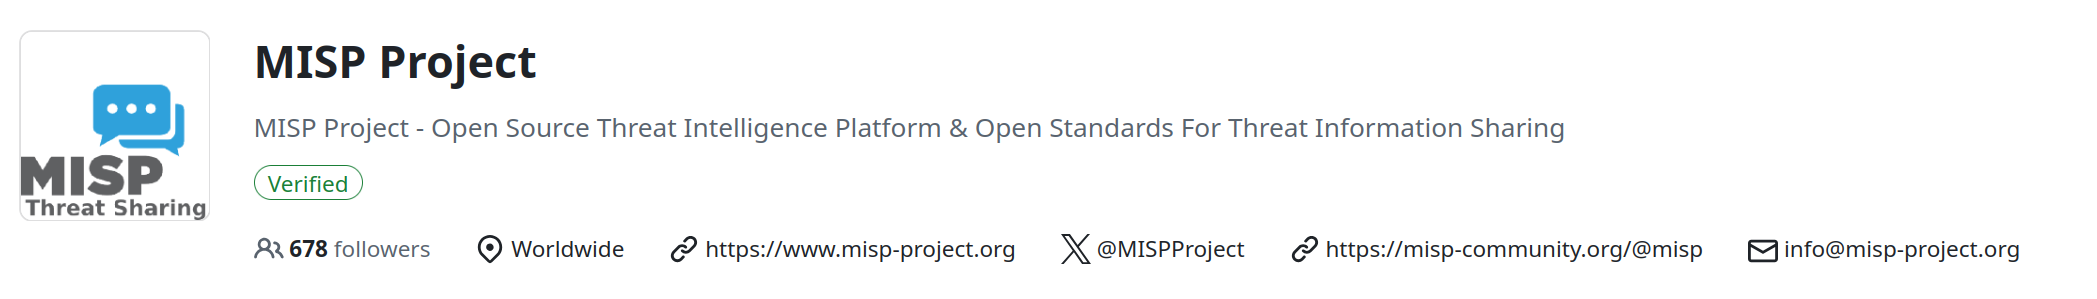
\includegraphics[width=1.0\textwidth]{misp-banner.png}
    \end{center}
    \begin{center}
            
\includegraphics[width=0.35\textwidth]{circl.png}
    \end{center}
    \begin{itemize}
            \item CIRCL is mandated by the Ministry of Economy
            \item CIRCL leads the development of MISP.
            \item {\bf CIRCL runs multiple large MISP communities performing active daily threat-intelligence sharing}.
            \item Funding is from LU, several EU programs and partnerships (EU/US) agreements.
    \end{itemize}
\end{frame}

\begin{frame}
    \frametitle{Plan of this session}
    \begin{itemize}
        \item MISP Intro: What it is, and what it can do
        \item Current state and Future of MISP
        \item How can MISP supports ISACs and its members
    \end{itemize}
    \vspace{1em}
    \begin{itemize}
        \item Building an information sharing community, lessons learnt and best practices\footnote{We published the complete guidelines in \url{https://www.x-isac.org/assets/images/guidelines_to_set-up_an_ISAC.pdf}}.
    \end{itemize}
\end{frame}

\begin{frame}
    \frametitle{What is MISP?}
    \begin{itemize}
        \item MISP is a {\bf threat information sharing platform} ({\bf TISP}) that is free \& open source software
        \item Mature project that was started in 2012, and since then, has been following a community-driven development
    \end{itemize}

    \begin{center}
        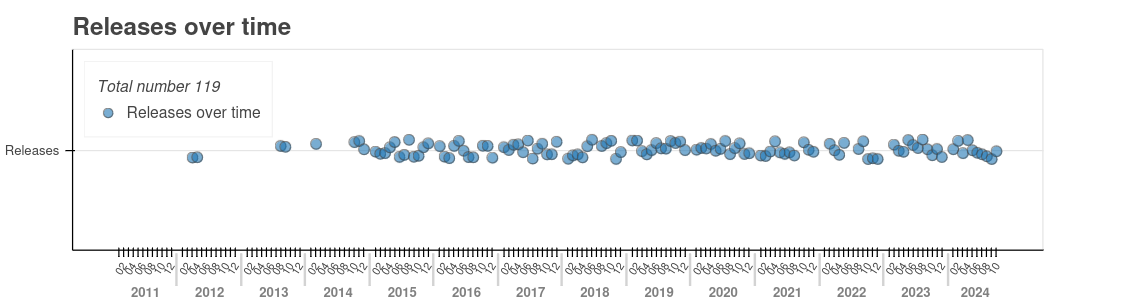
\includegraphics[width=0.99\linewidth]{release_overtime.png}
    \end{center}
\end{frame}

\begin{frame}
    \frametitle{What is MISP?}
    \begin{itemize}
        \item Used worldwide to share threat-related information
        \item \textbf{Open-source commitment}: Users of MISP can rely on the tool never turning into closed source
    \end{itemize}

    \begin{center}
        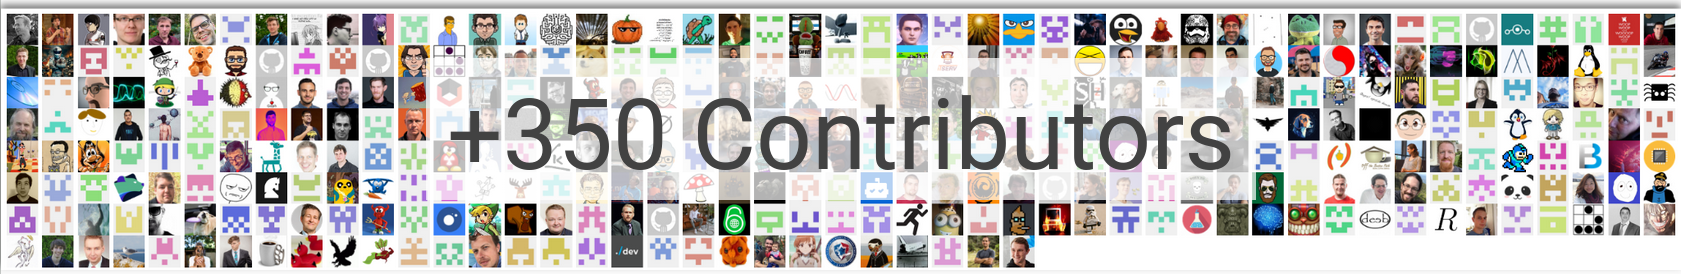
\includegraphics[width=0.99\linewidth]{contributors.png}
    \end{center}
\end{frame}

\begin{frame}
    \frametitle{What is MISP? (1)}
    \begin{itemize}
        \item MISP is a {\bf threat information sharing platform} ({\bf TISP}) that is free \& open source software
        \item A tool that {\bf collects} information from partners, your analysts, your tools, feeds
        \item Normalises, {\bf correlates}, {\bf enriches} the data
        \item Allows teams and communities to {\bf collaborate}
        \item {\bf Feeds} automated protective tools and analyst tools with the output
    \end{itemize}
\end{frame}

\begin{frame}
    \frametitle{Who is using MISP? (1)}
    \begin{center}
        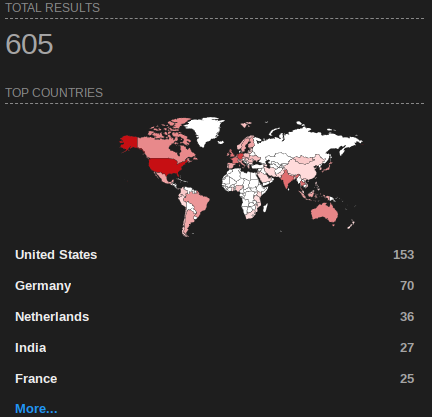
\includegraphics[scale=0.45]{misp-shodan.png}
        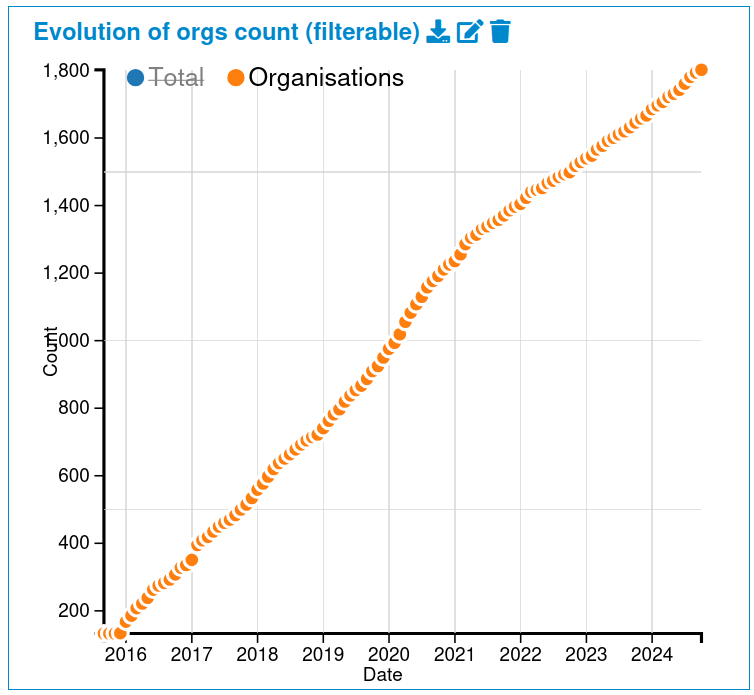
\includegraphics[scale=0.27]{org-count-misppriv.png}
    \end{center}
\end{frame}

\begin{frame}
    \frametitle{Who is using MISP? (2)}
    {\bf Communities:} groups of users sharing within a set of common objectives/values.
    \vspace{0.5em}
    \begin{itemize}
        \item {\bf Private sector} Financial, Manufacturing, Telecommunication
        \item {\bf Military and international organizations} (NATO, military CSIRTs, n/g CERTs,...).
        \item {\bf Security vendors} running their own communities (e.g. Fidelis) or interfacing with MISP communities (e.g. OTX).
        \item {\bf Topical communities} set up to tackle individual specific issues (COVID-19 MISP)
        \item {\bf ISACs} for many sectors (telecom, retail, aviations, ...) use MISP as a sharing mechanism
        \item {\bf Trusted groups} running MISP communities in island mode (air gapped system) or partially connected mode.
        \item {\bf LEA Agencies} EUROPOL, INTERPOL, MISP-LEA, $\cdots$
        \item {\bf International groups} FIRST.org, MISP-Priv, $\cdots$
    \end{itemize}
\end{frame}

\begin{frame}
    \frametitle{What is MISP? (2)}
    \begin{center}
        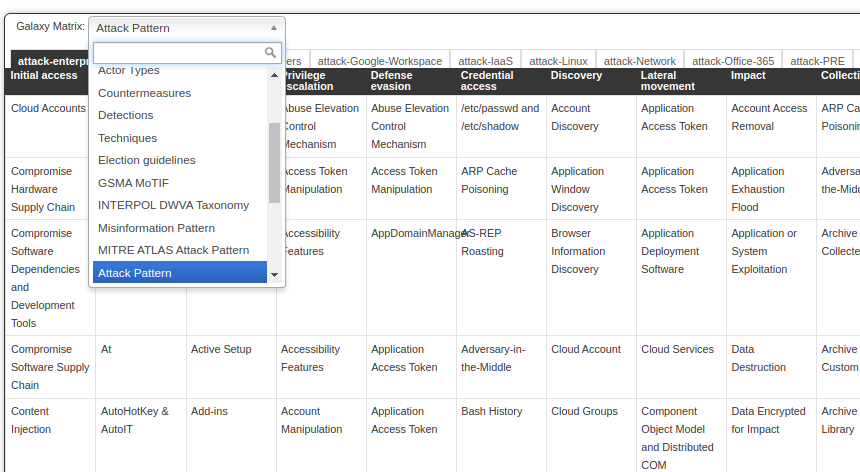
\includegraphics[width=1.0\linewidth]{galaxy-matrix.png}
    \end{center}
\end{frame}

\begin{frame}
    \frametitle{What is MISP? (2)}
    MISP is designed from the ground up to perform context-rich \textbf{threat intelligence}:
    \vspace{0.5em}
    \begin{itemize}
           \item {\bf Enrich} information with context and metadata
           \item Maps {\bf Threats and TTPs} (e.g MITRE ATT\&CK)
           \item Supports many {\bf standardized classification} marking
           \item Enables information {\bf curation} through automated quality checks
           \item Offers visualisation of threat {\bf relationships} and \textbf{technique} used
           \item Generates customizable {\bf threat reports}
           \item Allows creation of {\bf Dashboard} for trend analysis
    \end{itemize}
\end{frame}

\begin{frame}
    \frametitle{MISP Project Overview}
    \begin{center}
        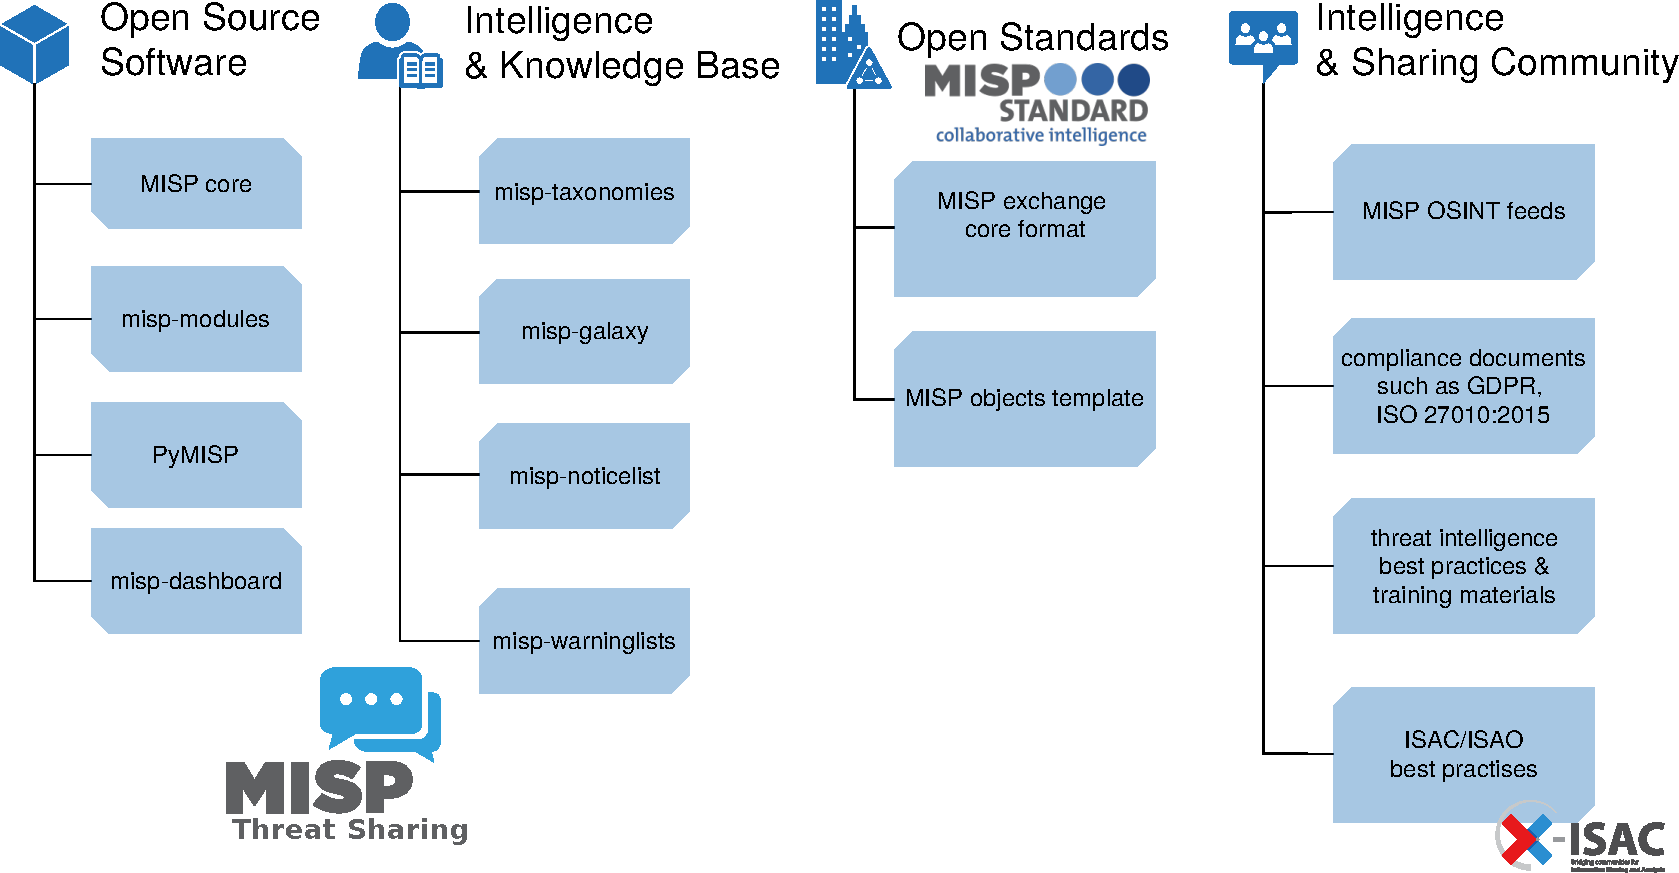
\includegraphics[width=0.85\linewidth]{misp-overview-simplified.pdf}
    \end{center}
\end{frame}


\begin{frame}
    \frametitle{Sharing in MISP (1)}
    \begin{center}
        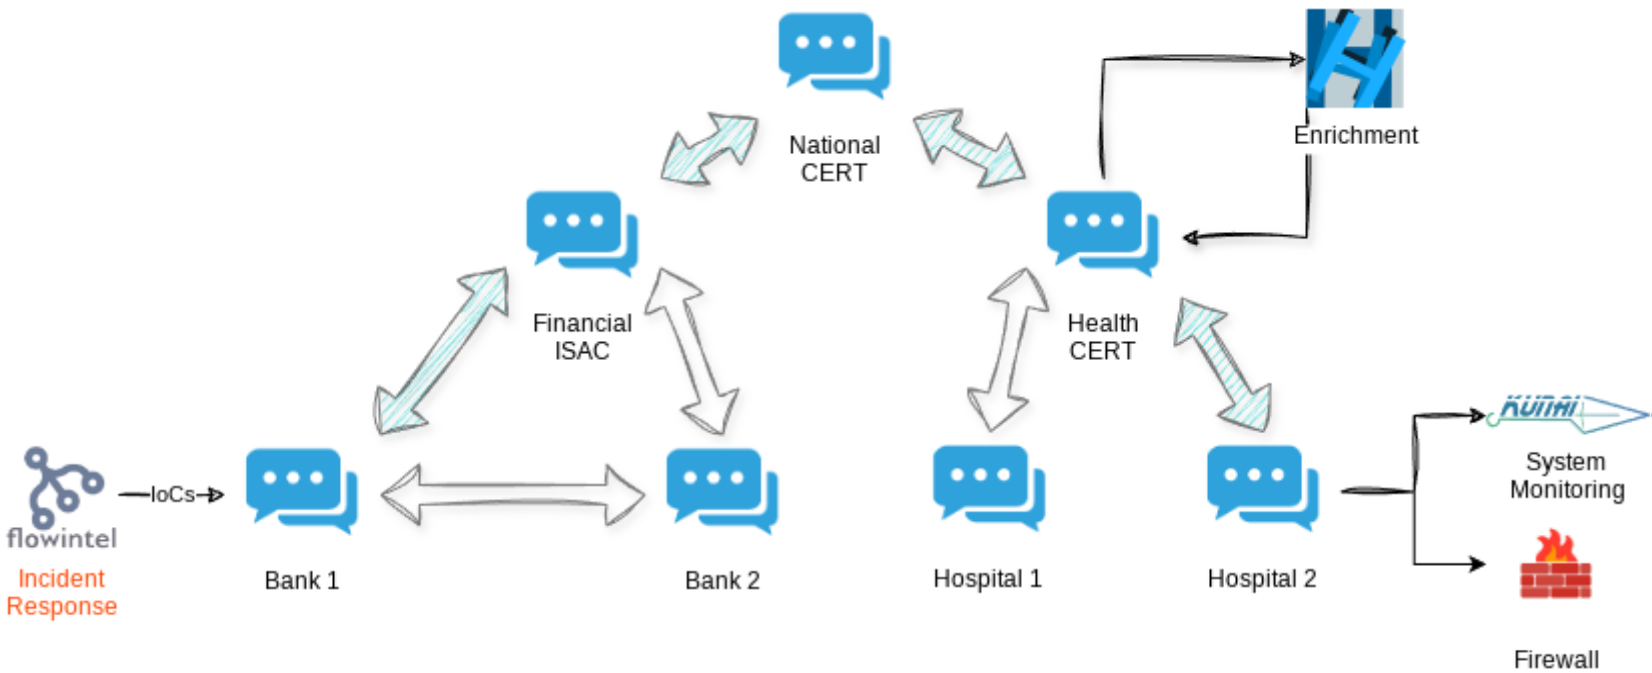
\includegraphics[width=0.99\linewidth]{misp-infosharing.png}
    \end{center}
\end{frame}

\begin{frame}
    \frametitle{Sharing in MISP (2)}
    MISP offers a wide range of \textbf{strategy to share information}:
    \begin{itemize}
        \item Many {\bf distribution level} offering granularity
        \item Sharing via distribution lists - {\bf Sharing groups}
        \item Incremental Synchronisation \& air-gapped sharing
        \item Feed system for ingestion \& generation
        \item User defined {\bf filtered sharing} for all the above mentioned methods
        \item Cross-instance information {\bf caching} for quick lookups of large data-sets
        \item Support for multi-MISP \textbf{internal enclaves}
    \end{itemize}
\end{frame}

\begin{frame}
    \frametitle{Information Quality Management}
    MISP has many features to help you manage and curate the data:
    \begin{itemize}
        \item \textbf{Correlating} data
        \item Feedback loop from detections via {\bf Sightings}
        \item {\bf False positive management} via the warninglist system
        \item {\bf Enrichment system} via MISP-modules
        \item {\bf Workflow} system to review and control information publication
        \item {\bf Integrations} with a plethora of tools and formats
        \item Flexible {\bf API} and support {\bf libraries} such as PyMISP to ease integration
        \item {\bf Timelines} and giving information a temporal context
        \item Full chain for {\bf indicator life-cycle management}
        \item {\bf Jupyter Notebooks} supporting common use-cases
    \end{itemize}
\end{frame}

\begin{frame}
    \frametitle{Integration and Automation ecosystem}
    MISP has many features to help you integrate various tools, processes and workflows:
    \begin{itemize}
        \item REST-full \textbf{API} \& \textbf{PyMISP}
        \item \textbf{PubSub channels} (ZeroMQ \& Kafka)
        \item \textbf{Enrichment} \& \textbf{Import/Export} service through MISP-modules
        \item \textbf{Workflow system}: Quick and easy automation based on trigger/conditions/actions blocks
    \end{itemize}
\end{frame}

\begin{frame}
    \frametitle{Information Quality Management}
    \begin{center}
        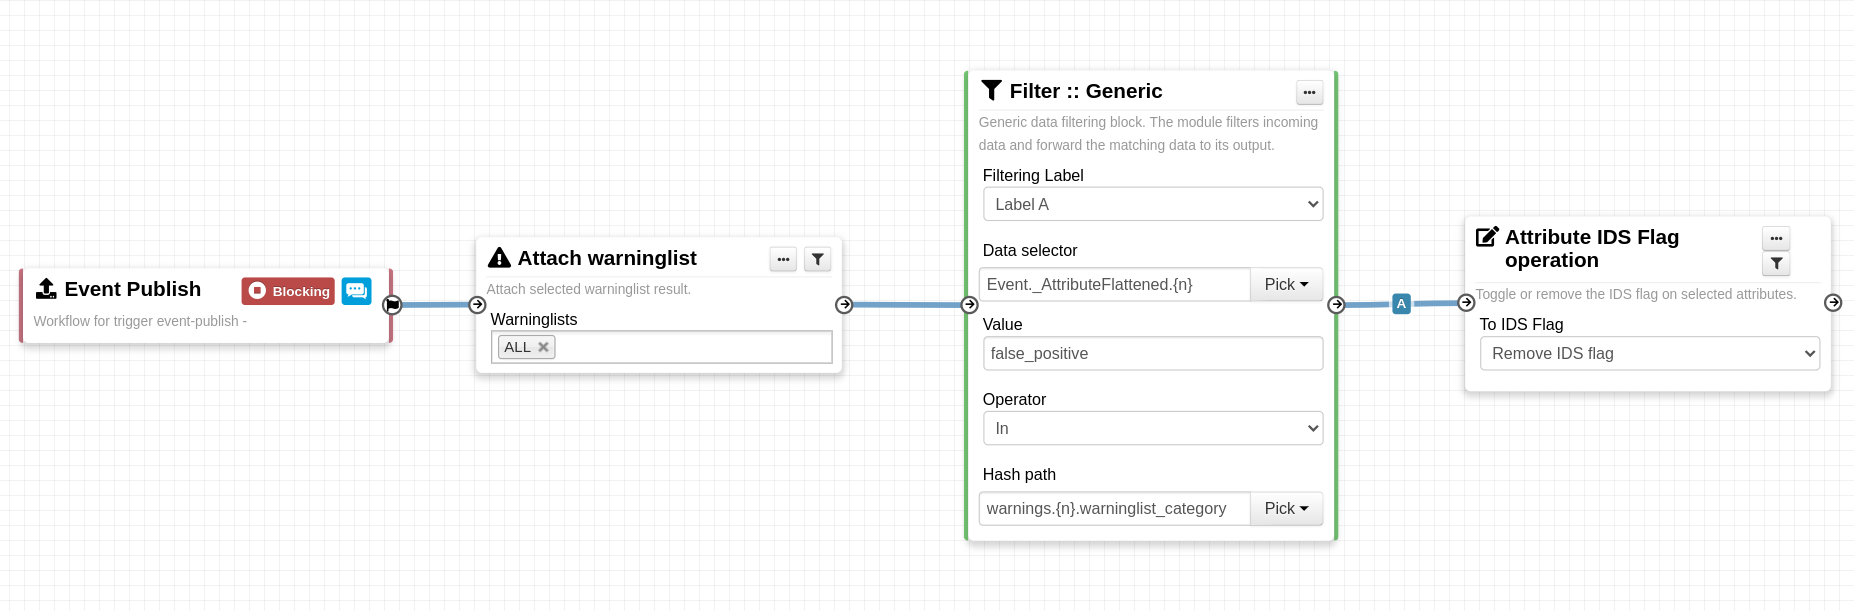
\includegraphics[width=0.99\linewidth]{wf-false-positive.png}
    \end{center}
    \begin{center}
        \textbf{Blueprint library} available on Github\footnote{\url{https://github.com/MISP/misp-workflow-blueprints}}
    \end{center}
\end{frame}

\begin{frame}
    \frametitle{Using the Power of the Community}
    MISP has many features to foster collaboration. To name a few:
    \begin{itemize}
        \item Proposals
        \item Analyst Data
        \item Delegation
        \item Sightings
        \item Extended Events
        \item Sharing-Groups
        \item $\cdots$
    \end{itemize}
\end{frame}

\begin{frame}
    \frametitle{Using the Power of the Community}
    \begin{center}
        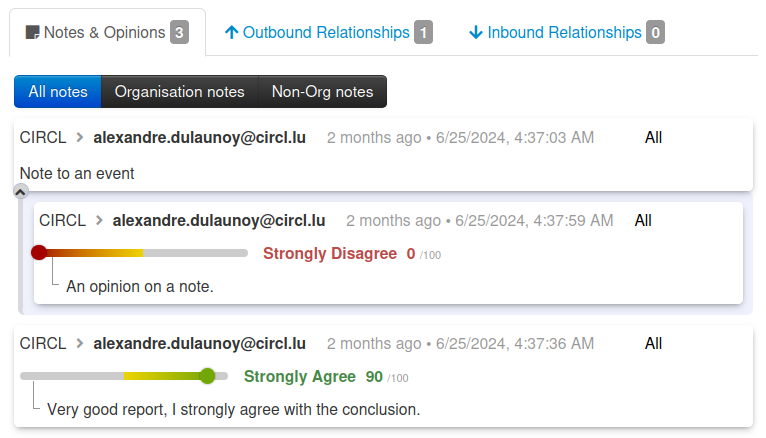
\includegraphics[width=0.85\linewidth]{analyst-data.png}
    \end{center}
\end{frame}

\begin{frame}
    \frametitle{Getting started: Joining/Running a sharing community using MISP}

    \begin{minipage}[t]{0.5\textwidth}
        \begin{center}
            \bf \Large As a Member
        \end{center}
        \begin{itemize}
            \item \textbf{Join} a "Hub" MISP instance
            \item \textbf{Host your own} MISP instance and connect to a "Hub"
        \end{itemize}
    \end{minipage}%
    \begin{minipage}[t]{0.5\textwidth}
        \begin{center}
            \bf \Large As a ISAC
        \end{center}
        Plan ahead:
        \begin{itemize}
            \item Estimate community \textbf{requirements and objectives}
            \item Decide on \textbf{common vocabularies}
            \item \textbf{Offer services} to your members
            \begin{itemize}
                \item Enrichment, Curation, $\cdots$
            \end{itemize}
        \end{itemize}
    \end{minipage}%
\end{frame}

\begin{frame}
    \frametitle{Success/Failure stories in MISP communities}
    TODO: To be added by alex
    \begin{itemize}
        \item CSSA
        \item Forced sharing as a requirement
    \end{itemize}
\end{frame}

\begin{frame}
    \frametitle{Advantage of MISP being free and open-source}
    TODO: To be added by alex
\end{frame}

\begin{frame}
    \frametitle{Future of MISP: What's ongoing}
    \begin{minipage}[t]{0.5\textwidth}
    \textbf{Medium term:}
    \begin{itemize}
        \item We just release a minor version \texttt{2.4}
        \item Support \texttt{2.4} until 6 months after \texttt{2.5}'s release
        \item Full feature parity and compatibility
        \item In progress: Installation/update scripts for alternate distros
    \end{itemize}
    \end{minipage}%
    \begin{minipage}[t]{0.5\textwidth}
    \textbf{Long term:} Major version \texttt{3.0}
    \begin{itemize}
        \item Purge old/unused functionalities
        \item Port of the codebase to a new stack
        \item Rework DB updates
        \item Revamp front-end \& aesthetics
        \item Analyst centric perspective
        \item Improved search and trend 
        \item Improved performance
    \end{itemize}
    \end{minipage}%
\end{frame}

\begin{frame}
    \frametitle{CIRCL's MISP Professional Services (MPS)}
    \begin{itemize}
        \item We are confortably funded for the project to continue to prospere
        \item MPS offers professional services \& supports the growth of the project
    \end{itemize}
    \vspace{1em}
    CIRCL's Offering:
    \begin{itemize}
        \item \textbf{Support Contract} - Prioritized resolution of issues and guidance
        \item \textbf{Training} - Adapted to the level of expertise of the participants
            \begin{itemize}
                \item {\small Free onboarding MISP training for ISACs and it's member}
            \end{itemize}
            \item \textbf{Hosting} - Hosted on our infrastructure (LU): Virtual or Dedicated
            \begin{itemize}
                \item {\small Maintenance of OS \& MISP, Early patching for security issues}
            \end{itemize}
    \end{itemize}
\end{frame}

\begin{frame}
    \frametitle{Conclusion}
    \begin{itemize}
            \item MISP is just a tool. What matters is your {\bf sharing practices}.
            \item MISP strives to meet any community's use-cases.
            \item MISP project combines {\bf open source softwares}, {\bf open standards \& best practices} to make information sharing a reality.
    \end{itemize}
\end{frame}



